\section{Method}
\label{sec:method}

In this section we present the theory applied in this work. 
we present our theoretical framework for expanding actor-critic RL algorithms with Ensemble methods.

\subsection{Generalized Critic}

We Actor-Critic

Actor  policy gradient method

Critic value function estimation

We introduce diversity through various ways

We average the 

\subsection{Variations}

Ensemble Learning is the foundation of the Generalized Critic method. The ability to introduce diversity in the models is therefore critical for functioning. 

The following are methods for introducing diversity into the models so that the final ensemble can average to something that may perform better than a single model. 

\subsubsection{Estimation methods for the value and advantage functions}

we can introduce diversity while estimating the advantage function.

we can uuse gae

we can use idk what ill check

also if we use gae we can change parameters
neat huh

%method
%gamma and lambda

\subsubsection{Random initialization and bootstrap at training}

The neural network estimator is initialized using random values, so as to diminish the noise produced by the initial values of a single model. When we train the network, we use a bootstrap\cite{efron1982jackknife} technique whereby at each update of the ensemble of value networks, we sample values from

\subsubsection{Hyperparameters and optimizations}



\label{sec:meth}
\begin{algorithm}[H]
\DontPrintSemicolon
  
  \KwInput{Initial actor network parameters $\theta_0$, initial critic parameter list $\phi^0_0, \dots, \phi^n_0$}
  %\KwOutput{Your output}
  %\KwData{Testing set $x$}

  \For{$i \leftarrow 1$ \KwTo total number of updates}{     
\While{buffer is not full}{     
  \tcc{collect set of trajectories $\mathcal{D}_k$}
         Run $\pi_{\theta_{old}}$ to generate an action
         
         Store the current state, action, and reward in buffer
         
         \If{episode ends}
         	{break}
   }
   
\If{episode was interrupted (buffer is full before episode end)}{
	\tcc{bootstrap remaining values}
	Run critic ensemble on last observation
	
	Combine estimates using the aggregation function
	
   }

  \For{$i \leftarrow 1$ \KwTo number of critics}{
   Estimate the advantage functions $\hat{A_i}$ using any (or several) estimation methods}

   Compute the PPO-CLIP policy loss as: %formula
   \[
   \theta_{k+1} = \argmax_{\theta} \frac{1}{\mathcal{D}_kT}\sum_{r \in |\mathcal{D}_k|}\sum^T_{t=0}\min \left(\frac{\pi_\theta(a_t|s_t)}{\pi_{\theta_k}(a_t|s_t)}A^{\pi_{\theta_k}}(s_t,a_t), g(\epsilon, A^{\pi_{\theta_k}}(s_t,a_t))\right)
   %{}{}
   \]
   
   Update the policy network

  \For{$i \leftarrow 1$ \KwTo number of critics}
    {
    	Update the value network $V_{\phi^1}$ by regression on mean-squared error:
    \[
    \Phi_{k+1} = \argmin_{\Phi} \frac{1}{|\mathcal{D}_k|T}\sum_{r\in \mathcal{D}_k}\sum^T_{t=0}\left(V_\Phi(s_t)-\hat{R_t}\right)^2
    \]
    }
}    
\caption{PPO-CLIP with Generalized Critic Policy Optimization}

\end{algorithm}

\begin{figure}[!htb]
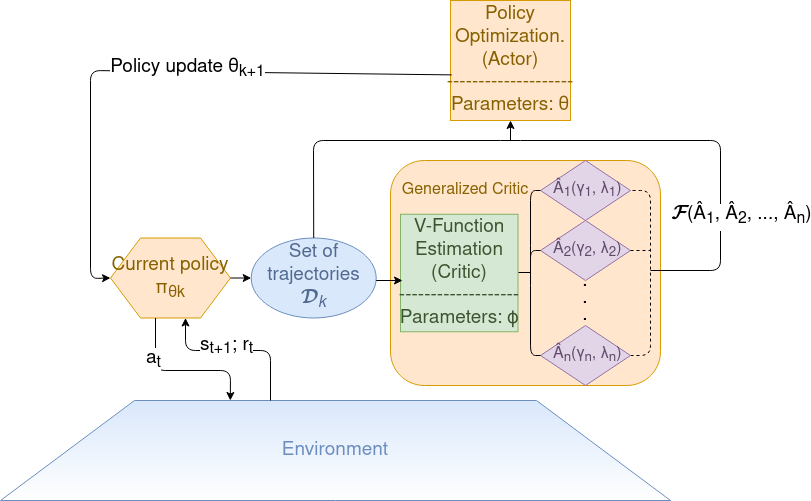
\includegraphics[width=\linewidth]{images/model}
\caption{Policy update scenario with a generalized critic.}
\label{fig:model}
\end{figure}


